\documentclass{myformat}
\addbibresource{mylib.bib}


% \makeglossaries

\setabbreviationstyle[acronym]{long-postshort-user}
\glssetcategoryattribute{acronym}{nohyperfirst}{true}
\setabbreviationstyle{short-nolong}
\makeglossaries

% --------------------
% ---- Glossaries ----
% --------------------
\newglossaryentry{asyncio}{name=Asyncio, description={A Python library for asynchronous code.}}
\newglossaryentry{stim}{name=STIM300, description={A MEMS-based \gls{imu}}}
\newglossaryentry{f9p}{name=F9P, description={A Global Navigation Satellite System (GNSS) receiver manufactured by u-blox.}}

% --------------------
% ----- Acronyms -----
% --------------------
\newacronym{asv}{ASV}{Autonomous Surface Vehicle}
\newacronym{dolp}{DoLP}{Degree of Linear Polarization}
\newacronym{aolp}{AoLP}{Angle of Linear Polarization}
\newacronym{sitaw}{SITAW}{Situational Awareness}
\newacronym{poe}{PoE}{Power over Ethernet}
\newacronym{pps}{PPS}{Pulse Per Second}
\newacronym{cpfa}{CPFA}{Color-Polarization Filter Array}
\newacronym{utc}{UTC}{Coordinated Universal Time}
\newacronym{imu}{IMU}{Inertial Measurement Unit}
\newacronym{tov}{TOV}{Time of Validity}
\newacronym{tm2}{TM2}{Time mark data}
\newacronym{gnss}{GNSS}{Global Navigation Satellite System}
\newacronym{ptp}{PTP}{Precision Time Protocol}

% \glsaddall
% \makenoidxglossaries

% \glsunset{cpu}
\glsunset{gnss}
\glsunset{imu}
\glsunset{tm2}
\glsunset{utc}

% --------------------
% ----- Shortcuts ----
% --------------------



\begin{document}


\title{Gaussian Splatting \\ A Significant Development in Novel View Synthesis}

\author{Emil Martens}
\markboth{Journal of \LaTeX\ Class Files,~Vol.~14, No.~8, August~2015}{}
\maketitle

\begin{abstract}
    The introduction of Gaussian Splatting has disrupted the field \gls{nvs} \cite{kerbl3DGaussianSplatting2023}. This technology has gained rapid adoption and further development in academia, and it has also been successfully leveraged in the industry, showcasing its immense potential \cite{LumaAIVideo}.

    This report aims to provide an accessible overview of the paper that introduced Gaussian Splatting and discuss its implications \cite{kerbl3DGaussianSplatting2023}.
    Additionally, we will look at certain areas where we believe the paper could have been improved.
    Finally, we will explore a hypothetical new method for \gls{nvs}, inspired by Gaussian Splatting, where we leverage the power of modern hardware-accelerated ray tracing.
\end{abstract}

\section{Introduction}
\gls{nvs} is a computer vision problem where the goal is to represent a scene in a way such that given a new \text{view}, an accurate image can be generated.
Here we define a \textit{view} as the position and orientation of a camera in the scene together with the camera's intrinsic parameters.

Current state-of-the-art methods vary in how they represent the scene and generate images
but share the same general problem formulation;
Given a set of training images $\bm{I}_i$,
taken from different views $\bm{V}_i$,
the goal is to find a representation of the scene $\bm{S}$,
together with a image generating, i.e. rendering, function $\bm{\hat{I}}_i = g(\bm{S}, \bm{V}_i)$,
such that some cost function $\mathcal{L}(\bm{I}_i, \bm{\hat{I}}_i)$,
is minimized over all training images.

To evaluate the performance of a method, a collection of test images $\bm{I}_j$ together with their corresponding views $\bm{V}_j$ is used to evaluate the method's ability to generalize to unseen data.
Beyond a method's ability to accurately generate images from novel views, other important metrics should be considered.
This includes the time it takes to generate an image, the memory required to store the scene representation, the time it takes to train the model, the amount of training data required and the amount of memory required during training.



\subsection{Related Works}
\gls{nvs} is a well-studied problem in computer vision, and many different approaches have been proposed.
Older methods achieved decent image interpolation by estimating the depth of the scene to correctly warp and blend adjacent images \cite{zitnickHighqualityVideoView2004}.

A big leap in performance was achieved with the introduction of \gls{nerf} methods, where a continuous representation of the scene is built by optimizing a neural network to predict the color and opacity at any point in the scene given a direction \cite{mildenhallNeRFRepresentingScenes2020a}.
A severe limitation of this approach however is the amount of time it takes to train the model, partially because a lot of resources are wasted on rendering transparent or occluded parts of the scene, as the whole volume is sampled.

Plenoxels dropped the costly neural network and instead represented the scene using a sparse voxel grid \cite{yuPlenoxelsRadianceFields2021a}.
Point sampling is still used but is now calculated by blending the values stored in the vertices of the voxel grid, resulting in a significant speedup. Spherical harmonics are used to represent the view-dependent color of each voxel \cite{yuPlenoxelsRadianceFields2021a}.

Related to this, Instant Neural Graphics introduced using multiple voxel grids at different levels of detail and a multi-level hash table to look up the closest vertices \cite{mullerInstantNeuralGraphics2022}.
They also optimized two \glspl{mpl} together with the vertex values to give the opacity and color of each voxel \cite{mullerInstantNeuralGraphics2022}.

None of the previous methods are very similar to Gaussian Splatting but are still relevant as they are the current state-of-the-art methods for \gls{nvs}.






\section{Paper Summary}
This section gives a summary of the method presented in the paper, outlined in Figure \ref{fig:pipeline},
with an emphasis on explaining concepts that did not receive a lot of attention in the paper.

\begin{figure*}
    \centering
    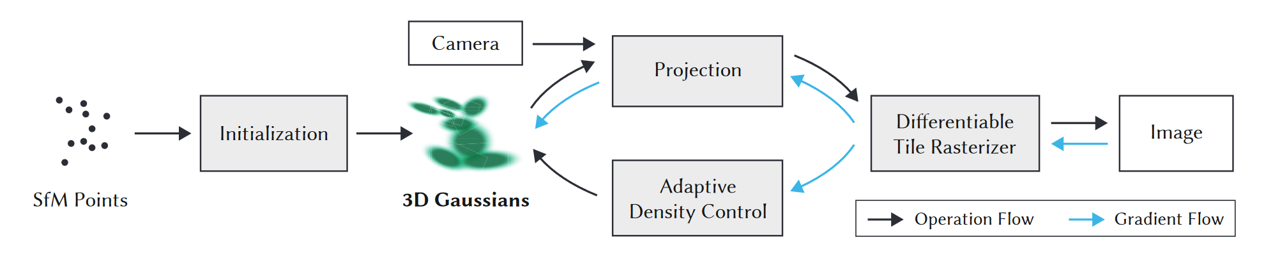
\includegraphics[width=\textwidth]{images/pipeline.png}
    \caption{The Gaussian splatting pipeline presented in the paper \cite[Fig. 2]{kerbl3DGaussianSplatting2023}.}
    \label{fig:pipeline}
\end{figure*}


\subsection{Representation}
The core idea of the paper is to represent the scene as a set of Gaussians.
Each Gaussian is defined by its position $\bm{\mu}$, its covariance matrix $\bm{\Sigma}$, its opacity $\alpha$ and its spherical harmonic coefficients $\bm{c}$ used to give it a view-dependent color, further discussed in Section \ref{sec:spherical_harmonics}.
The covariance is defined as
\begin{align}
    \bm{\Sigma} = \bm{R} \bm{S} \bm{S}^T \bm{R}^T,
\end{align}
where $\bm{R}$ is a rotation matrix stored as a quaternion $\bm{q}$ and $\bm{S}$ is a diagonal matrix containing the standard deviation of the Gaussian along each axis, stored as a vector $\bm{s}$.
To ensure that the covariance is positive definite, the values of $\bm{s}$ are passed through a sigmoid activation function, and quaternion $\bm{q}$ is normalized to ensure a proper rotation matrix.
In total, each Gaussian has 59 parameters, 3 for the position, 3 for the scale, 4 for the quaternion 1 for alpha and 48 for the spherical harmonic coefficients.

\subsection{Spherical Harmonics}
The first step in the rendering process, which is sort of overlooked in the paper, is to calculate the color of each Gaussian for a given view direction.
This is done using spherical harmonics, which can be seen as a spherical equivalent of the discrete cosine transform.
A key advantage of spherical harmonics is that they are differentiable and continuous.


\subsection{Projection}
\label{sec:projection}
The next step of the rendering pipeline, shown in Figure \ref{fig:pipeline}, is to project the Gaussians onto the image plane.
First, the Gaussians are transformed into the camera frame using a linear view transformation $\bm{W}$.
Then the Gaussians are projected onto the image plane using a pinhole projection.
This transformation is visualized by comparing Figure \ref{fig:proj_2a} and Figure \ref{fig:proj_2b}.


\begin{figure}[t]
    \centering
    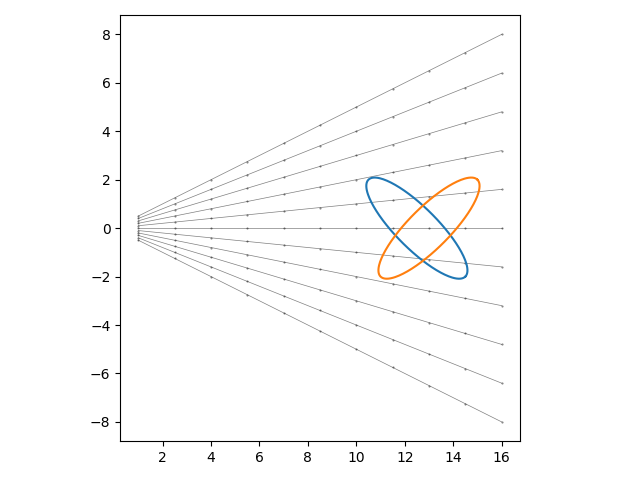
\includegraphics[width=\linewidth]{images/proja.png}
    \caption{Covariance ellipses of two Gaussians in the camera frame viewed from the side, with visualization of pixel rays.}
    \label{fig:proj_2a}
\end{figure}


Two key steps are performed to speed up the projection process.
First, instead of accurately projecting the Gaussians onto the image plane, a linear approximation is used where the center point is projected properly, but the covariance is updated given the following linear approximation,
\begin{align}
    \bm{\Sigma'} & = \bm{J} \bm{W} \bm{\Sigma} \bm{W}^T \bm{J}^T \label{eq:linear_approx}
\end{align}
where $\bm{J}$ is the Jacobian of the projection function.
The result of this approximation is visualized as the two dotted ellipses in Figure \ref{fig:proj_2b}.

A second significant speedup step is to flatten the projected Gaussians by only looking at their first two dimensions, resulting in 2D Gaussian with position $\bm{\mu}''$ and covariance $\bm{\Sigma}''$, visualized as a line in Figure \ref{fig:proj_2b}.
The key benefit of this is that the depth ordering of the Gaussians is identical for each pixel, which would not be the case otherwise as seen in Figure \ref{fig:proj_2b}.
This does however introduce a significant problem, where small changes in view direction can decide which Gaussian is in front of another Gaussian, resulting in strong popping artifacts, which the paper acknowledges \cite[Sec 7.4]{kerbl3DGaussianSplatting2023}.

\begin{figure}[htb]
    \centering
    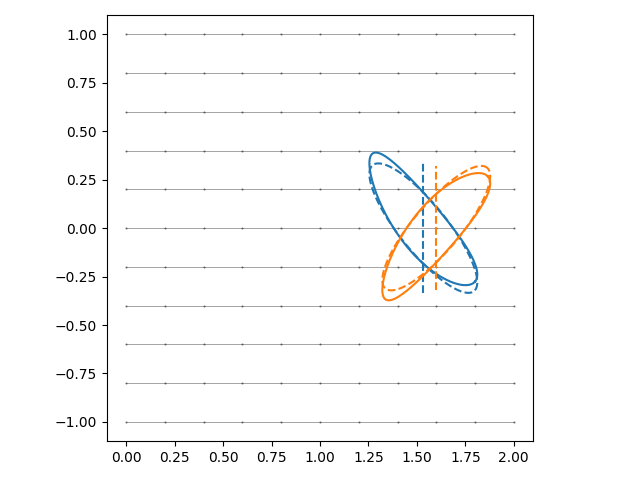
\includegraphics[width=\linewidth]{images/projb.png}
    \caption{The camera projection of Figure \ref{fig:proj_2a}. The dotted lines are the linear approximation of the Gaussians given Equation \ref{eq:linear_approx} and the vertical line is the simplification from removing the depth component}.
    \label{fig:proj_2b}
\end{figure}


\subsection{Rasterization Pipeline}
\label{sec:rasterization}
After the projection is complete, we have a set of 2D Gaussians that need to be rendered.
To achieve high frame rates, the paper uses a rasterization pipeline where the output image first is divided into 265 blocks.
Then they check which blocks each projected Gaussian overlaps with by drawing a circle with a radius of three times the largest eigenvalue of the covariance matrix, as illustrated in Figure \ref{fig:rendering}.
Gaussians outside the image plane or with a size smaller than one pixel are discarded, e.g. Gaussian D and E in Figure \ref{fig:rendering}
Then, they duplicate each Gaussian for each block it overlaps with and sort the Gaussians, first, according to the block they belong to and then according to their depth value.
This sorting is performed only once per iteration and they combine the block-index bits and depth bits into a single integer to perform both sorts in a single pass using parallel radix sort.

Each block is then responsible for non-overlapping sequential sections of the sorted output.
The color of each rendered pixel is calculated by iterating over the Gaussians in the block and blending them together using the alpha blending function given by
\begin{align}
    C   & = \sum_{i \in N} c_i a_i \prod_{j=1}^{i-1} (1-a_j)                                                     \\
    a_i & = \alpha_i \cdot exp(-\frac{1}{2}(\bm{x}-\bm{\mu}''_i)^T \bm{\Sigma}{''}_i^{-1} (\bm{x}-\bm{\mu}''_i))
    \label{eq:alpha_blending}
\end{align}
where $C$ is the resulting color, $c_i$ is the color of the $i$'th Gaussian calculated from the view direction and its spherical harmonic coefficients and $a_i$ is the evaluated opacity.

\begin{figure}
    \centering
    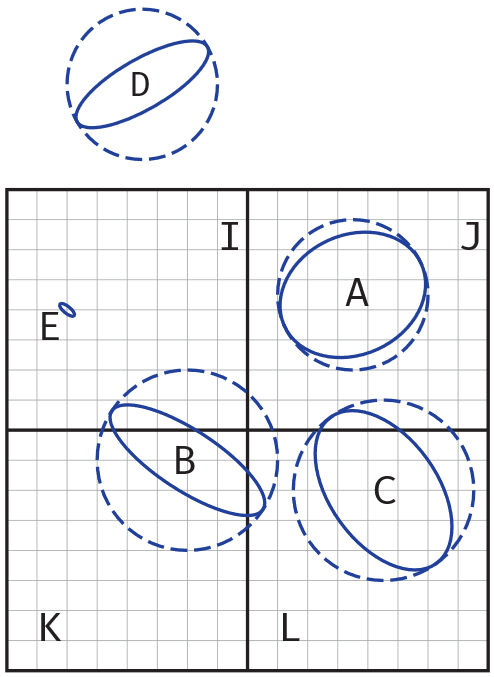
\includegraphics[width=0.6\linewidth]{images/rendering.png}
    \caption{Visualization of how Gaussian splats are rendered using multiple independent blocks. The dotted lines are from drawing a circle with a radius of three times the largest eigenvalue of the covariance matrix.}
    \label{fig:rendering}
\end{figure}


\subsection{Backpropagation}
The paper L1 loss together with structural dissimilarity index (D-SSIM) loss.
\begin{align}
    \mathcal{L} = (1 - \lambda) \mathcal{L}_1 + \lambda \mathcal{L}_{D-SSIM}
\end{align}
They have implemented custom CUDA accelerated backward pass functions for both the rasterization, projection and spherical harmonics steps that utilize cached information from the forward pass for speedup.



\subsection{Densification and Pruning}
In the paper, they use adaptive density control to generate Gaussians in areas where they are needed and remove unnecessary Gaussians to reduce memory usage.

For both the densification methods they simply check if a Gaussian has had large gradients with respect to position, i.e. if they have moved a lot around over the past 300 iterations.
They argue this happens when the Gaussian is moving to an area that is underrepresented or if the Gaussian is to big to fit the area it is in \cite[Sec 5.2]{kerbl3DGaussianSplatting2023}.
If the Gaussian is smaller than a certain threshold, it is cloned, and if it is larger than a certain threshold, it is split into two smaller Gaussians, as shown in Figure \ref{fig:densification}.

\begin{figure}
    \centering
    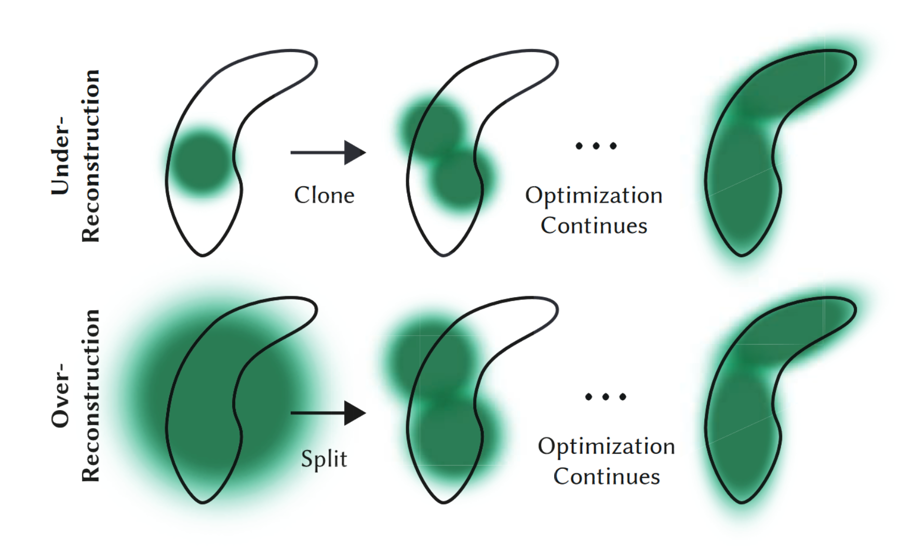
\includegraphics[width=\linewidth]{images/densification.png}
    \caption{The adaptive Gaussian densification scheme presented in the paper \cite[Fig. 4]{kerbl3DGaussianSplatting2023}.}
    \label{fig:densification}
\end{figure}

\section{Critique and Potential Improvements}
While the paper presents a very impressive method for \gls{nvs}, there are certain areas where we believe the method can improve.



% \begin{figure}
%     \centering
%     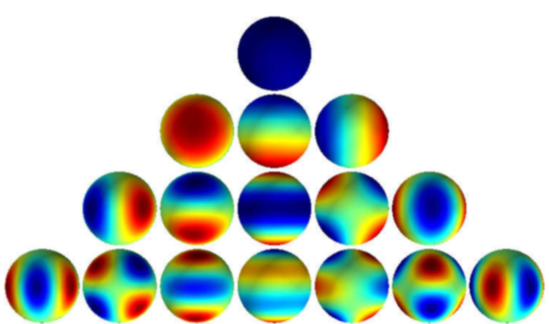
\includegraphics[width=\linewidth]{images/spherical_harmonics.png}
%     \label{fig:spherical_harmonics}
%     \caption{Visualization of the spherical harmonics used to represent the view-dependent color of each Gaussian \cite{pokorny2014a}.}
% \end{figure}

\subsection{Use CUDA Streams to increase parallelism}
The code provided by the authors showcases a deep understanding of CUDA and GPU architecture,
notably in the way they ensure memory coalescing, avoid bank conflicts and leverage shared memory in the rasterization pipeline.
This makes it surprising that they do not use CUDA streams to increase parallelism.
When training the scene on a workstation with an i9-13900KF CPU and an RTX 4090 GPU the GPU utilization was only around 30\% as the training process was severely bottlenecked by the single-threaded CPU code.
In the paper, they acknowledge that the majority (\textasciitilde 80\%) of the training time is spent in Python code, and argue it is a tradeoff to allow for easy adoption by other researchers \cite[Sec. 8]{kerbl3DGaussianSplatting2023}.
While the adaptability of the code is appreciated, it does not explain why they did not use CUDA Streams to increase parallelism, as Streams have deep support in PyTorch and can easily be disabled even if support is implemented \cite{pytorchcontributorsCUDASemanticsPyTorch2023}.

\subsection{Regularization}
The paper acknowledges that the optimized Gaussians tend to be very non-isotropic, i.e. very stretched out, as  Regularization is not performed \cite[Sec. 7.4]{kerbl3DGaussianSplatting2023}.
This is illustrated in Figure \ref{fig:very_isotropic}.
One way to solve this would be to add a cost based on the index of dispersion of the scale parameters $\bm{s}$ of each Gaussian, that is the ratio of the variance to the mean, which would have a value of 0 for spherical Gaussians.

\begin{figure}
    \centering
    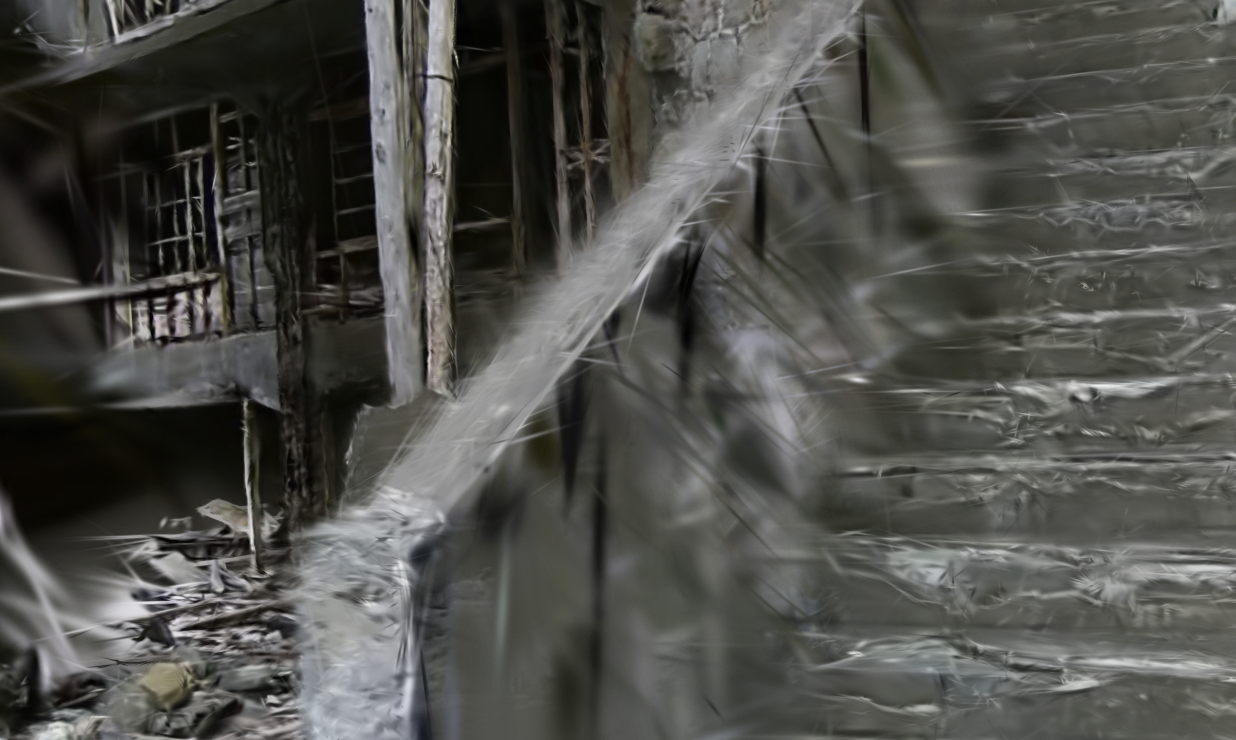
\includegraphics[width=\linewidth]{images/very_isotropic.png}
    \caption{Going outside the captured view angles illustrate how non-isotropic the Gaussians are \cite{@nekoHashimaIslandCreated2023}}
    \label{fig:very_isotropic}
\end{figure}

\subsection{Faster Opacity Calculation}
% Why they chose to use a Gaussian to represent the scene is not clearly explained in the paper.
In the current implementation, they evaluate the exponential function for each pixel for each Gaussian in the pixel's block, which is computationally expensive.
A threshold based on the Mahalanobis distance can be used to avoid this exponential calculation for most Gaussians.
\begin{align}
    m_i & =\frac{1}{2}(\bm{x}-\bm{\mu}''_i)^T \bm{\Sigma}{''}_i^{-1} (\bm{x}-\bm{\mu}''_i) \\
    a_i & =\begin{cases}
               0 \alpha_i \cdot exp(-\frac{1}{2}m_i) & \text{if } m_i \leq 3^2 \\
               0                                     & \text{if } m_i  > 3^2
           \end{cases}
\end{align}
Using a polynomial density function with shorter tails, e.g. $(1-x^2)^2$ instead of the exponential function would result in fewer tiny gradients, and avoid calling the expensive exponential function, probably resulting in a speedup.
With the current implementation being severely bottlenecked by the CPU code, this might not have a significant impact.



\subsection{Replace Spherical Harmonics}
\label{sec:spherical_harmonics}
In the current implementation, they use spherical harmonics to handle view-dependent color from reflections.
They present this approach as "following standard practice" referencing the Plenoxels and Instant Neural Graphics papers \cite{yuPlenoxelsRadianceFields2021a}\cite{mullerInstantNeuralGraphics2022}.
As the paper uses a fundamentally different representation of the scene, using the same approach for view-dependent color might not be the best choice.

The other methods both use some voxel-based representation of the scene,
where the sampling of each point is independent of the view direction,
making it necessary for each point to contain view-dependent color \cite{yuPlenoxelsRadianceFields2021a}\cite{mullerInstantNeuralGraphics2022}.
In the Gaussian splatting method, a discrete set of Gaussians is used to represent the scene, which could be leveraged to avoid the need for view dependence by having overlapping Gaussians with view-dependent opacity.
This could be used to have Gaussians that are only visible from a narrow range of view directions, placed in front of the scene geometry to simulate reflections.

The paper shows that even without spherical harmonics, the scene converges to a good result \cite[Table 3]{kerbl3DGaussianSplatting2023}.
We propose to remove the spherical harmonic coefficients from the representation of each Gaussian, reducing the parameter number from 59 to 14, altering the cost function and adding a second phase to the rendering pipeline to handle reflections.
As reflections add light to the scene, we can penalize the cost of the rendered image more if it is too dark than if it is too bright.
After convergence, we can add a second optimization step where the converged scene is kept constant and additional Gaussians with view-dependent opacity can be added to add highlights to reflective surfaces. A potential problem with this approach is however the popping effect discussed in Section \ref{sec:projection}, which makes it difficult to optimize overlapping Gaussians.
\section{A New Approach}
While the Gaussian splatting method is very impressive, this section will discuss a potential new path for \gls{nvs} inspired by the Gaussian splatting method.
The core idea is to leverage the power of hardware-accelerated ray tracing and replace the current rasterization pipeline with a ray tracing pipeline.
Additionally, the use of polarization cameras might prove useful in this regard, as reflected light has a distinct polarization signature \cite{lingUniversityPhysicsVolume2016}.

\subsection{Ray Tracing}
Ray tracing is a rendering technique that simulates how rays of light traverse a scene.
Unlike rasterization, which confines rendering to a single viewpoint at a time by projecting the scene onto a two-dimensional image plane, ray tracing can simultaneously render rays originating from multiple viewpoints \cite{caulfieldWhatPathTracing2022}.
This capability lets ray tracing programs simulate lifelike lighting scenarios by estimating how light scatters and reflects off objects in the scene \cite{caulfieldWhatPathTracing2022}.

As ray tracing has become a key component of rendering in the video game industry, specialized hardware has been developed to accelerate the process to achieve real-time performance.
Modern NVIDIA GPUs have dedicated \gls{rt} cores that can be used to accelerate ray tracing through the NVIDIA OptiX\textsuperscript{TM} API \cite{nvidiaNVIDIAOptiXProgramming2023}.

The main computational bottleneck of ray tracing is finding the intersections between the rays and the scene geometry.
To speed up this process, a \gls{bvh} is used to store the scene geometry \cite{nvidiaNVIDIAOptiXProgramming2023}.
A \gls{bvh} is a tree data structure that recursively divides the scene into smaller and smaller bounding boxes making it possible to quickly discard large parts of the scene that the ray does not intersect with \cite{nvidiaNVIDIAOptiXProgramming2023}.
The \gls{rt} cores are specialized hardware that can traverse the \gls{bvh} and find intersections between rays and scene objects very fast \cite{nvidiaNVIDIAOptiXProgramming2023}.


\subsection{Triangle Representation}
While Optix supports custom primitive types, making the use of Gaussians possible, operations on custom primitives are only partially accelerated by the \gls{rt} cores \cite{nvidiaOptiXQuickStart2018}\cite{nvidiaNVIDIAOptiXProgramming2023}.
This makes the use of triangles a more attractive option.
The implementation in the paper projects the Gaussians onto the image plane, i.e. they are not performing any volumetric rendering,
making it likely that using triangles also should be possible.

Instead of storing position, orientation and scale parameters, we can store the position color and opacity of the three vertices of the triangle.
This representation is simpler than the Gaussian representation and removes the necessity for activation functions used to ensure a positive definite covariance matrix.
The density function of each triangle can be calculated using the barycentric coordinates of the intersection point, as this is supplied by Optix \cite{nvidiaNVIDIAOptiXProgramming2023}.
Several different polynomial-based functions have been tested to obtain a smooth opacity function, as shown in Figure \ref{fig:alphas}.

Hypothetically, it could be possible to use meshes instead of individual triangles, that is multiple triangles sharing the same vertices, as this is also supported by Optix \cite{nvidiaNVIDIAOptiXProgramming2023}.
This will make a scene representation more compact but will make the optimization problem more complex.


\begin{figure}
    \centering
    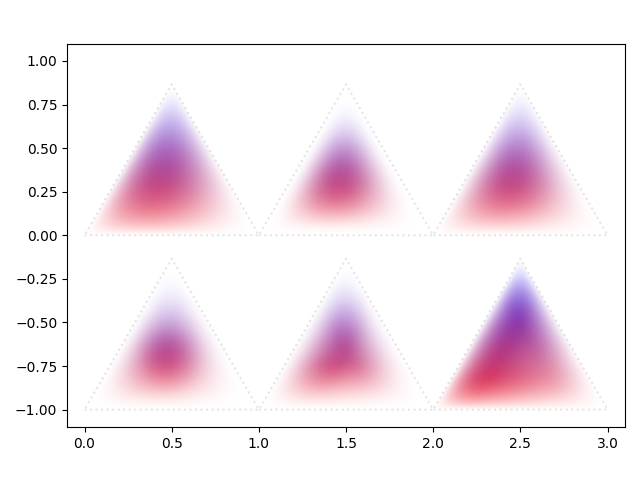
\includegraphics[width=\linewidth]{images/alphas.png}
    \caption{Experimentation with different polynomial functions on barycentric coordinate values to obtain a smooth opacity function. The lower right vertex of each triangle has opacity 0 to test vertex-dependent opacity.}
    \label{fig:alphas}
\end{figure}

\subsection{Program Structure}
The program structure will be similar to the current implementation, with a few key differences.
As ray tracing is used, there is no need for any projection step as described in Section \ref{sec:projection}.
The rendering process for each pixel in the paper will be matched by a rendering process for each ray in the new implementation, using the same blending function as described in Equation \ref{eq:alpha_blending}.

The optimization process will however be different.
During the rendering process, information about each intersection will be captured and stored in a buffer.
Taking inspiration from the paper, after the rendering passes the collection of intersections can be sorted by the index of the triangle they intersect with.
Then for each triangle, an optimization function can be defined based on the collection of intersections with that triangle.
Having information about all the intersections on each triangle can be leveraged to perform smarter optimization steps, as illustrated in Figure \ref{fig:optimization}.



\begin{figure}
    \centering
    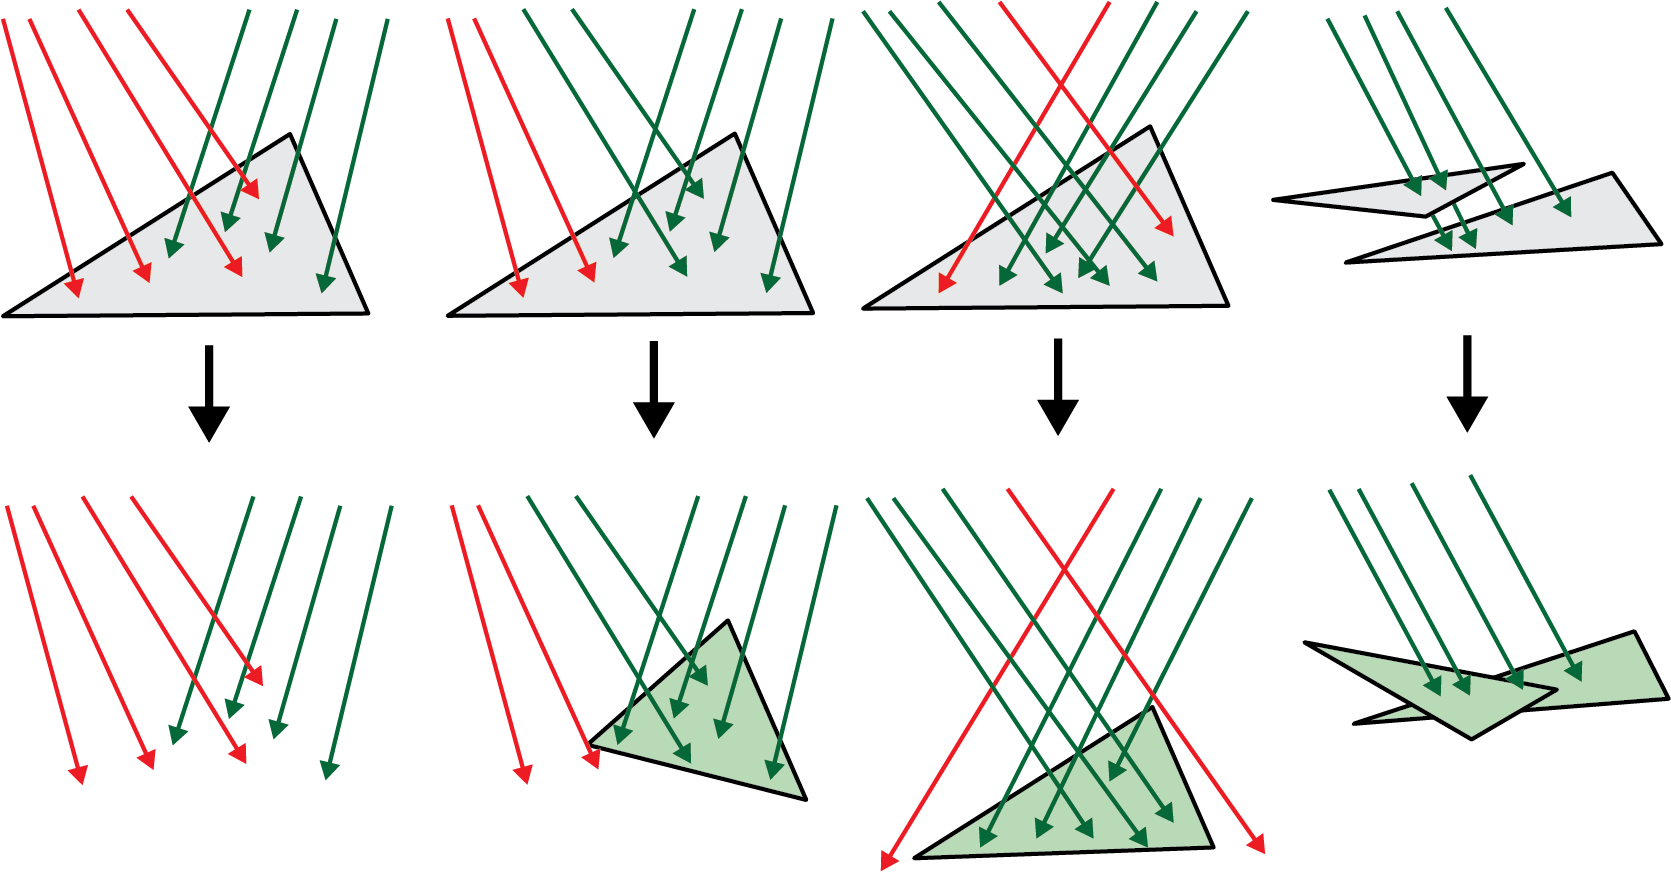
\includegraphics[width=\linewidth]{images/optimization.png}
    \caption{Four illustrative examples of how intersection information can be used to delete, reshape move and regularize triangles. The color of the rays is the color of the pixel from which it originates.}
    \label{fig:optimization}
\end{figure}

\subsection{Remove Popping Artifacts}
As discussed, a key issue with the current implementation is popping artifacts where Gaussians suddenly appear or disappear behind other Gaussians.
Raytracing will solve most of this issue as the projection approximation described in Section \ref{sec:projection} is no longer needed.
Still, in the intersection area between two triangles, the gradients will be discontinuous due to how alpha blending works, as shown in Equation \ref{eq:alpha_blending}.

A potential approach to solving this, achieving a smooth transition when triangles move through each other,
is to use a dynamic alpha blending function where the ray distance between the current triangle intersection and the next triangle intersection is taken into account.
This will however create a lot of dependence between the triangles, as the alpha value of each triangle is dependent on the alpha value of the next triangle which is dependent on the alpha value of the next triangle and so on.

\subsection{Inter Triangle Regularization}
A key benefit of capturing the intersections between rays and triangles is that we can perform inter-triangle regularization.
For each intersection point with a triangle, we can capture information about the distance and color of the previous and next intersection points.
If the distances are within some adaptive threshold, we can add a regularization term to the loss function, such that neighboring triangles should stick together.
Hopefully, this will help towards having smoother surfaces and aligning the face normal of neighboring triangles.
This is illustrated in the rightmost example in Figure \ref{fig:optimization}.

\subsection{Reflections}
Reflections in the scene pose a significant challenge in the field of \gls{nvs}, as it requires the ability to capture view-dependent color.
As discussed earlier, the use of spherical harmonics solves this to some degree, but it comes at a significant memory cost.
When using ray tracing, it might be possible to circumvent the need for view-dependent color by using ray-traced reflections.

Without the use of ray tracing cores, this is impossible, as the whole rendering pipeline for the Gaussian splats, discussed in Section \ref{sec:rasterization}, would have to be performed for each reflected ray as they would not share the same origin.
This would make the rendering process several million times slower.
But with the use of ray tracing cores, rendering a reflected ray is no different than rendering a regular ray \footnote{It might be slightly worse due to data locality, but this should be handled by the hardware.}.

It is however still very likely that it is infeasible to optimize the scene with reflections.
A core reason for this is that it is very expensive to capture glossy reflections, such as light reflected from a table surface, as statistical sampling with a large number of sample rays is required to get a good result.
Another key challenge is that a very small change in the orientation of a triangle can have large effects on the reflected light, resulting in very sharp gradients.


\subsection{Leverage Polarization}
Using polarization cameras might be a way to circumvent the need for view-dependent color.
The simple approach would be to remove reflected light from the scene.
This approach only targets the input data and should thus be easy to evaluate using the implementation from the paper.
The results from this approach will however look different than what a regular camera would capture, as the reflected light is partially removed.

Another, arguably more interesting, approach would be to use the polarization information to estimate the surface normal of each triangle and calculate ray-traced reflections.
As the polarization cameras can capture the angle of polarization for each pixel, using multiple views it should be possible to estimate the three-dimensional surface normals with some degree of accuracy.
This approach has been presented by one manufacturer of polarization cameras as shown in Figure \ref{fig:polarization} \cite{lucidvisionlabs3DDepthSurface2021}.

def
\begin{figure}
    \centering
    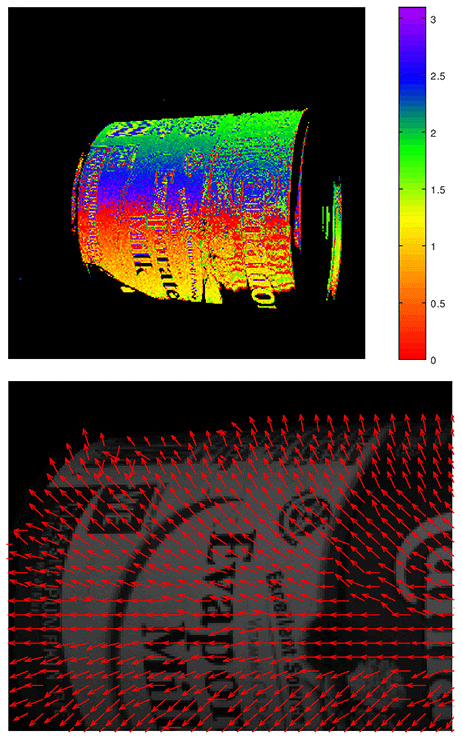
\includegraphics[width=.9\linewidth]{images/polarization_normals.png}
    \caption{Angle of orientation and estimated surface normals from polarized light \cite{lucidvisionlabs3DDepthSurface2021}}.
    \label{fig:polarization}
\end{figure}

\section{Conclusion and Future Work}
In this paper we have presented a new portable sensor rig design we believe will make collecting sensor data in maritime environments significantly easier.

If you are interested in


We currently only provide raw datasets from the sensor rig, as our calibration results needs further validation, but we plan to release a calibrated dataset with fused position estimates in the future.


\printglossary[type=\acronymtype]
% \printglossaries
\printbibliography

\end{document}